\documentclass[12pt]{article}
\usepackage{amsmath}
\usepackage{amssymb}
\usepackage{graphicx}
\usepackage{tabulary}
\usepackage{textcomp}


\begin{document}

\title{Roll Control for LV2.3}
\author{William Harrington\\ %Nate: if you edit this document, please include your name next to mine
\textit{Portland State Aerospace Society}}
 
\maketitle

\begin{description}
	\item[Introduction] \hfill \\
		The roll control system for the current generation of launch vehicle (2.3) has more or less not been functioning properly since Launch 8. \textbf{Nate: explain here some of the problems with previous incarnations of the roll control system that led up to where we are now}. In June of 2014, another attempt at designing a roll control system was initiated. The purpose of this report is to document the process of re-developing the roll control system.
		
\end{description}

\begin{description}
	\item[Physics Models] \hfill \\
	In this section we examine the equations for the physical phenomenon of our dynamic system.\\
	
	The angular acceleration due the canards
	\begin{equation}
		\ddot{\theta} = \frac{4Lr}{I}
	\end{equation}
	Where L represents Lift, and r represents the canard distance from the Z axis.\\
	
	Lift is defined as
	\begin{equation}
		L = \frac{1}{2}C_{L}\rho v^2 S
	\end{equation}
	Where $C_{L}$ represents the coefficient of lift, $\rho$ is air density, v is velocity, and $S = 11.64cm^2$ is the area of a canard.\\
	
	The air density $\rho$ is defined by a basic exponential atmosphere model that depends on altitude. We use the model below:
	\begin{equation}
		1.225e^{-0.000119h}
	\end{equation}
	
	The coefficient of lift is broken up into two categories: supersonic flow and subsonic flow. For subsonic flow it is defined as
	\begin{equation}
		C_{L} = K_{p} cos^2(\alpha) sin(\alpha) + K_{v} cos(\alpha) sin^2(\alpha)
	\end{equation}
	And for supersonic flow it conveniently shrinks to
	\begin{equation}
		C_{L} = \alpha K_{v}
	\end{equation}
	Where $K_{p} \approx 2.45$, $K_{v} \approx 3.2$, and $\alpha$ is the angle of the canard which is physically restricted to be between $\pm15$\textdegree.
	
\end{description}
 
\begin{description} 
	\item[State space model] \hfill \\
		In this section we set out to develop a state space model for the roll dynamics of the rocket. \\
		
		Modern control theory is founded on the state space approach. Therefore, we will review and discuss important terminology that pertains to developing our state space model. \\
			 
		The \textbf{state} of a dynamic system is the smallest set of variables (called \textit{state variables}) such that knowledge of these variables at $t = t_{0}$, together with knowledge of the input for $ t \geq t_{0}$, completely determines the behavior of the system for any time $t \geq t_{0}$. \cite{MCE}\\
			
		The \textbf{state variables} of a dynamic system are the variables making up the smallest set of variables that determine the state of the dynamic system. If at least \textit{n} variables \textit{$x_{1}, x_{2},..., x_{n}$} are needed to completely describe the behavior of a dynamic system (so that once the input is given for $t \geq t_{0}$ and the initial state at $t = t_{0}$ is specified, the future state of the system is completely determined), then such \textit{n} variables are a set of state variables. \cite{MCE}\\
			
		If \textit{n} state variables are needed to completely describe the behavior of a given system, then these \textit{n} state variables can be considered the \textit{n} components of a veto \textbf{x}. Such a vector is called a \textbf{state vector}. A state vector is thus a vector that determines uniquely the system \textbf{x(t)} for any time $t \geq t_{0}$, once the state at $t = t_{0}$ is given and the input \textbf{u(t)} for $t \geq t_{0}$ is specified. \cite{MCE} \\
			
		The \textit{n}-dimensional space whose coordinate axes consist of the \textit{$x_{1}$} axis, \textit{$x_{2}$} axis,..., \textit{$x_{n}$} axis, where \textit{$x_{1}, x_{2},..., x_{n}$} are state variables, is called a \textbf{state space}. Any state can be represented by a point in the state space. \cite{MCE} \\
			
		The equations for the most general state-space representation of a linear system with \textit{p} inputs, \textit{q} outputs and \textit{n} state variables below:\\
			\begin{equation}
				\dot{\textbf{x(t)}} = A(t)\textbf{x(t)} + B(t)\textbf{u(t)}\\
			\end{equation}
			\begin{equation}
				\textbf{y(t)} = C(t)\textbf{x(t)} + D(t)\textbf{u(t)}\\
			\end{equation}

		\item [Deriving the state space equations] \hfill \\
		Equations approximating the motion of the rocket are derived from free-body diagrams (FBD) and kinetic diagrams (KD), as taught in a mid level mechanical engineering dynamics course. Developing equations in this manner is known as developing from first principles because basic Newtonian principles $F=ma$ are used to derive them. \cite{PSAS} \\
		
		The diagrams are shown below:
		\begin{itemize}
			\item[] 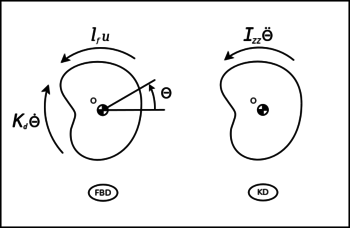
\includegraphics[scale=.5]{350x250-RollFBD.png} \\
			
				\textit{From this diagram we get the following differential equation}\\
				\textit{$I_{zz}\ddot{\theta} = l_{f}u - K_{d}\dot{\theta}$} \cite{PSAS} \\
			
			\item[]

				%\textit{Blahblah} \\
				
		\end{itemize}
		
\end{description}
 
\newpage
 \begin{thebibliography}{9}
 \bibitem{PSAS}
 Portland State Aerospace Society, Roll Control Wiki
 \texttt{http://psas.pdx.edu/rollcontrol/}
 \bibitem{MCE}
 Katsuhiko Ogata
 \textit{Modern Control Engineering, Fifth Edition}
 Prentice Hall, Boston, MA, 2010
 \end{thebibliography}
\end{document}
